%\chapter{det-comp}


%%%%%%%%%%%%%%%%%%%%%%%%%%%%%%%%%%%%%%%%%%%%%%
%\section{Anode Plane Assemblies}

%%%%%%%%%%%%%%%%%%%%%%%%%%%%%%%%%%%%%%%%%%%%%%
\section{Cathode Plane Assemblies}


\subsection{Scope, Requirements and Design Considerations}

The cathode plane is located in the middle of the TPC, dividing it into two equal distance drift volumes.  It is connected to the high voltage feedthrough through a receptacle, aka the HV cup, at the east end, and biased at -180\,kV.  The cathode plane is constructed from 6$\times$3 cathode plane assemblies (CPAs) to form the 7\,m $\times$ 6\,m area.  It provides the bias voltage and current to all the field cage modules (top, bottom and end wall) through electrical interconnects.  It also mechanically supports 6 pairs of top/bottom field cage modules.
The cathode plane is suspended by insulating bars from the CPA installation rail.



%%%%%%%%%%%%%%%%%%%%%%%%%
\subsubsection{Requirements}
%The principal requirements on the CPA are as follows. It is required to do the following:
The CPA is required to:
\begin{itemize}
\item provide equipotential surfaces at $-$180kV nominal bias voltage,
\item maintain a flatness better than 1~cm when submerged in the liquid argon,
\item be constructed of materials with comparable CTEs to that of stainless steel, 
\fixme{CTE coeff of therm expansion -- add to acronym list}
\item limit the electric field exposed to LAr to under 30~kV/cm 
\item prevent damage to the TPC, including its readout electronics, in case of a HV discharge anywhere on the cathode,
\item provide constant bias voltage and current to all attached field cage (FC) resistor divider chains,
\item support the full weight of the 4 connected top/bottom field cage modules plus a person on the bottom CPA during installation,
\item accommodate cryostat roof movement between warm and LAr-filled states,
\item be constructed in a modular form that can be easily installed in the cryostat,
\item accommodate PD calibration features, and
\item avoid any trapped volume.
\end{itemize}

%%%%%%%%%%%%%%%%%%%%%%%%%
\subsection{Design Considerations}

In each single phase DUNE far detector, the cathode planes are 12m tall by nearly 60m long.  When biased to the nominal voltage of -180kV, each cathode plane stores more than 100\,J of energy. It is of great concern on the integrity of the detector elements, including the sensitive front end electronics, if this energy is suddenly and completely released in a high voltage discharge event.  Study has shown (DUNE docdb 1320) that if the entire cathode plane is made of interconnected metallic electrodes, there is significant risk of damage to the front end ASICs simply due to the charge injection through the capacitive coupling between the cathode and the anode wires when the cathode voltage is force to ground by a high voltage discharge.  

Since  a large fraction of the stored energy on the cathode plane is determined by the operating voltage and the drift distance, reducing the drift distance and therefore the cathode voltage is an option.  However, doing so while maintaining a constant detector fiducial volume would require additional detector elements and increase cost and complexity of the system.  And this will not reduce the amount of charge injection since the voltage-capacitance product remains nearly constant between the anode and cathode planes.

Subdividing the cathode into electrically isolated partitions also reduces the total energy from a single cathode partition. However the capacitive coupling between wires and cathode will not change substantially until the partition size is comparable to the drift distance. Multiple HV feedthroughs and ports per cathode also increases the system complexity. Complete HV isolation of the cathode segments is a difficult task to achieve, if we also want the cathode plane to have little distortion in the drift field during normal operation of the detector. 

The solution adopted in the single phase TPC design is to make the entire cathode plane out of highly resistive material such that the entire cathode has a very long discharge time constant compared to an all metal construction.  In an event of high voltage breakdown at any given location on the cathode, the sudden change in voltage only occurs in a relatively localized area.  The rest of the cathode surface maintains its original bias voltage, and gradually discharge to ground through the large resistivity of the cathode material.  This greatly reduces the instantaneous charge injection to the front end electronics.

In the single phase DUNE FD, two cathode planes are positioned roughly at 1/4 and 3/4 of the width of the TPC.  Since the cathode planes are not at the geometrical center of the cryostat, the thermal convection flow of the liquid argon will exert an unbalanced force on each cathode plane. Computerized Fluid Dynamic (CFD) study (E. Voirin FD CFD) shows that a pressure differential on the cathode plane of the order of $\sim$1 pascal is to be expected.  The cathode plane must be designed to withstand such pressure without exceeding the 1cm flatness requirement.




%%%%%%%%%%%%%%%%%%%%%%%%%
\subsection{The Design of the Cathode}

%%%%%%%%%%%%%%%%%%%%%%%%%
\subsubsection{Overview}

The cathode design has evolved through several iterations over the years.  The design chosen for the ProtoDUNE TPC is an array of moderately sized modules constructed from strong G10 frames holding thin G10 sheets laminated with a commercial resistive Kapton film on both sides.   Compared with the size of an APA, the CPA modules are 1/2 in width (1.16m) and 1/3 in height (2m).   Each module has four G10 bars holding a 3mm thick G10 sheet with resistive coating.  The thickness of the G10 bars is 6cm.  The surfaces of the bars facing the APAs are covered by another set of resistive G10 strip with a different bias voltage such that these G10 bars does not cause any distortion in the drift field beyond the resistive surfaces.

The 3 modules forming a single column are rigidly bolted together.  Each column is suspended to the CPA support rail by a single insulating G10 bar.  On the top and bottom edges of this CPA column, there are two hinges supporting the partial weight of the top and bottom field cage modules.   Adjacent columns are aligned through pin and slot connections to maintain co-planarity while allowing minor relative vertical shift due to cryostat roof movement.

The electrical connectivity of the resistive panels along each vertical column is maintained by several tabs through the edge frames.  Across the columns, there is no direction electrical connection between the panels.  Instead, they are interconnected by the "high voltage bus". 

The high voltage bus is a loop of a high voltage cable placed along the outer edges of the entire CPA plane, hidden between the field shaping strip overhang and the main cathode resistive sheet.  This cable must be capable of withstanding the full cathode bias voltage to prevent direct arching to (and as a result, recharging) a cathode panel having a discharge to ground. The HV bus makes redundant connections to the resistive panels across columns.  It also provide a low resistance path for the field cage resistive divider chains around the cathode edges.

The outer edges of the cathode plane facing the cryostat wall are populated with the same metal profiles with insulating polyethylene caps used in the field cage.  This eliminated the need for a special design of the most crucial edges of the cathode plane: the edges of the CPA now look just like the continuation of the field cage.  Since these profiles are the only objects facing grounded surfaces, they are the most likely candidates to have HV discharges to ground.   To limit peak current flow, these edge profiles are resistively connected to the main cathode panels through their laminated resistive surfaces.  


\begin{cdrfigure}[Resistive surface CPA Concept]{cpa-concept}{The resistive surface CPA concept. 
 Left: A 3D model of a corner of the cathode showing major components;  Right: E field simulation of a portion of the cathode.} 
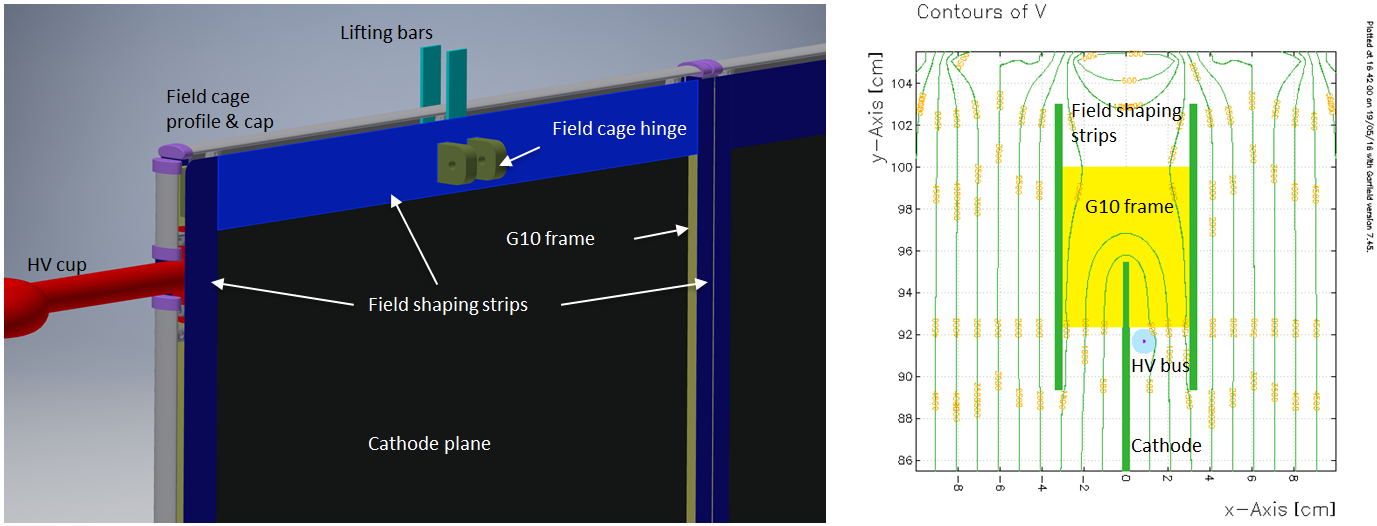
\includegraphics[width=\linewidth]{tpc_cpa_concept.png}
\end{cdrfigure}


%%%%%%%%%%%%%
\subsubsection{Resistive material}
%% from F. Pietropaolo

The main criteria for the selection of the resistive material to be used for the CPA panels are: 
\begin{itemize}	
\item surface resistivity range,
\item compatibility with cryogenic temperatures,
\item robustness to HV discharges, 
\item material ageing,
\item radio-purity,
\item availability on large area, and \fixme{what does this mean?}
\item achievable level of planarity. 
\end{itemize}

Several options have been evaluated, with the following characteristics:
\begin{itemize}	
\item NORPLEX Micarta NP 315, phenolic laminate loaded with graphite: Intrinsic bulk resistivity in the required range (few M$\Omega$/cm); density comparable to LAr;
\item Screen printed resistive ink on G10/FR4 substrate (~100 k$\Omega$/square) printed with specific patterns to obtain required average surface resistivity;
\item DuPont resistive Kapton film  (25 $\mu$m thickness, graphite loaded, available with resistivity in the 0.5 to 50 M$\Omega$/square range) laminated on G10/FR4 substrate.
\end{itemize}
Also considered at earlier stage were
\begin{itemize}	
\item Zelec ESD powder mixed with polyurethane binder, and
\item ESD surface conducting G10 from Current Composite.
\end{itemize}

 Radiological tests performed at the LNGS low-counting-rate facility indicate that G10/FR4 is preferable; for most relevant radioactive chains, MiCarta is more active by orders of magnitude.

Screen-printed resistive ink and Kapton lamination on G10/FR4 are both well established fabrication techniques available on panels as large as to 2.1$\times$1.2 m$^2$ (well matched to the CPA panel's required size). The resistive ink technique allows to choose precisely the average surface resistivity value by tailoring the printed line width and pattern, while Kapton exhibits an uniform surface coverage. 


Tests on large-size panels have demonstrated that both options can withstand repeated immersions in LAr without deformation or delamination. The increase in resistivity that occurs at LAr temperature is limited to less than a factor two for both. Electrical contacts for both surfaces are made with a silver paint paste that is highly stable at LAr temperature and resistant to mechanical scratches.
%
However, results of tests for surface ageing when exposed to HV sparks indicate that Kapton is the preferred solution:
\begin{itemize}	


\item For the resistive ink, sparks tend to propagate along the direction of less resistivity, perpendicular to strip direction. This induces a visible degradation of the material surface with some  ink evaporation and measurable local changes in resistivity (Figure~\ref{fig:cpa-resink}).
\item For the Kapton, sparks induce tiny points of carbonization on the material surface, but do not appear to change the average resistivity (Figure~\ref{fig:cpa-kapton}). 
\end{itemize}


\begin{cdrfigure}[Resistive ink ageing from sparks]{cpa-resink}{Resistive ink ageing from sparks. 
 {\bf Left:} spark propagation along preferred directions (lower resistivity), {\bf Right:} Status after test: degradation with some material evaporation.} 
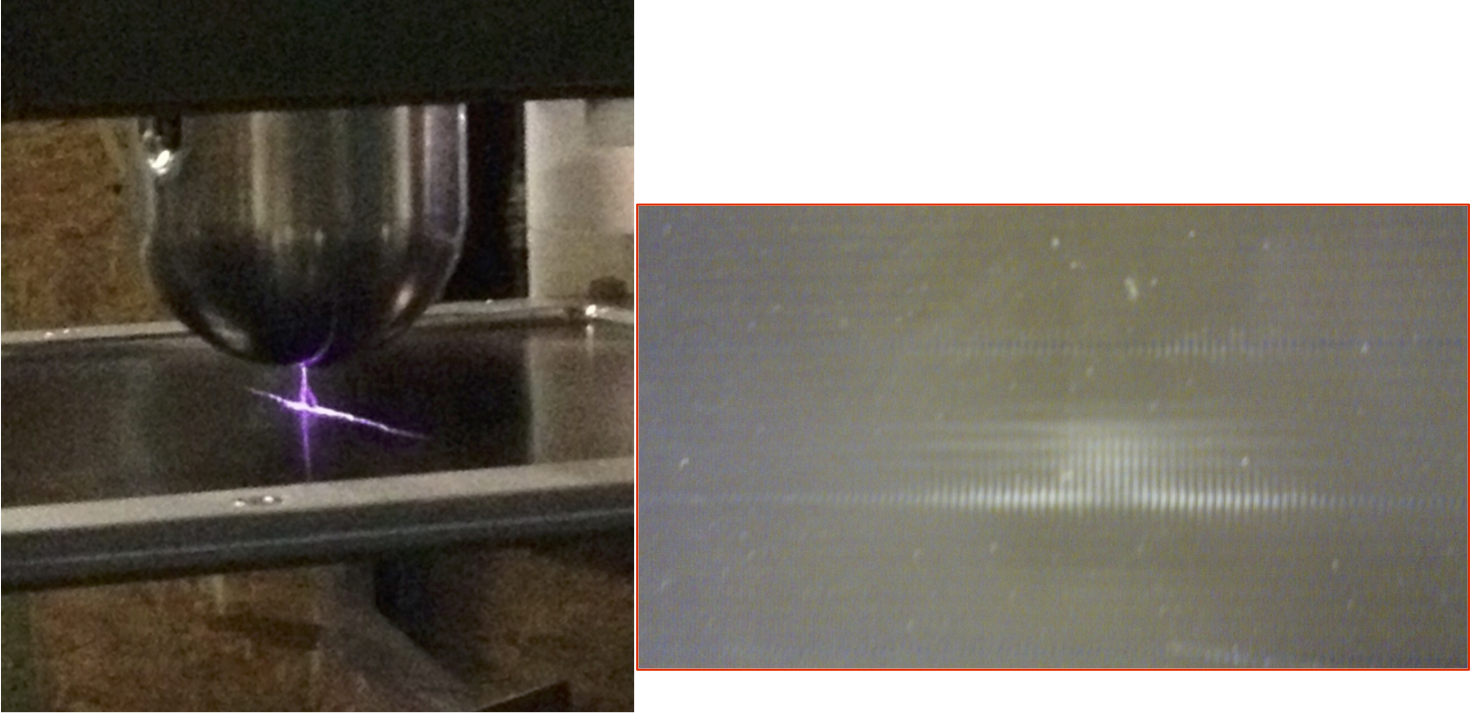
\includegraphics[width=\linewidth]{tpc_cpa-resink.png}
\end{cdrfigure}

\begin{cdrfigure}[The field cage test setup]{cpa-kapton}{Resistive kapton ageing from sparks. 
 {\bf Left:} point-like sparks. {\bf Right:} Localized carbonization on material surface, at the spark position.}
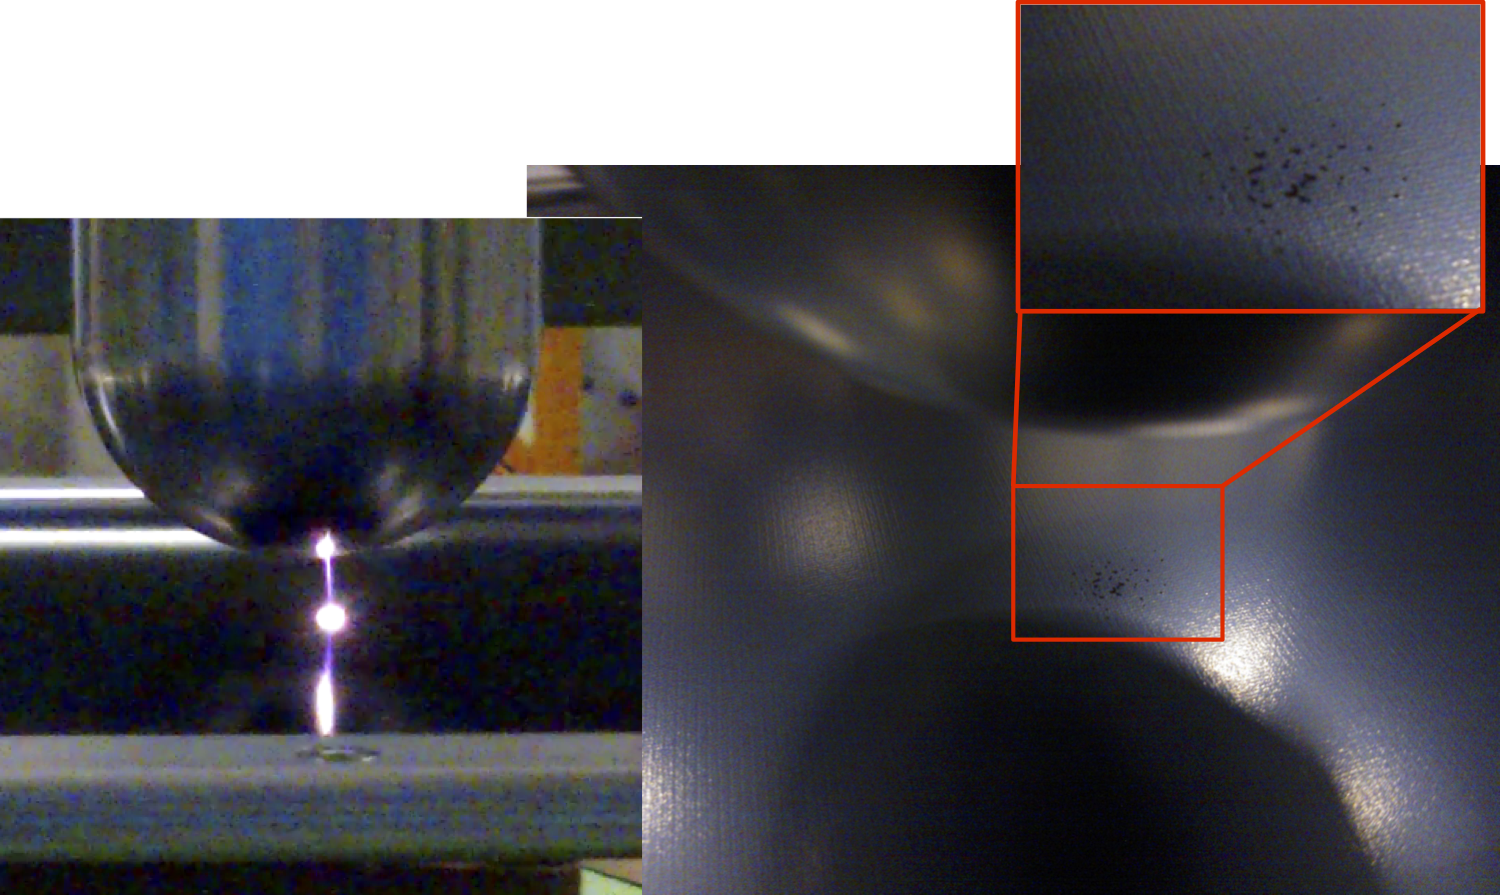
\includegraphics[width=\linewidth]{tpc_cpa-kapton.png}
\end{cdrfigure}

%%%%%%%%%%%%
\subsubsection{Support frame material properties}

The main materials for the detector are stainless steel and what is called generically G10 material.  G10 is a thermosetting industrial fiber glass composite laminate consisting of a continuous filament glass cloth material with an epoxy resin binder. This product, first introduced in the 1950's, has characteristics of high strength, low moisture absorption, excellent electrical properties  and chemical resistance. These properties are maintained not only at room temperature but also under humid or moist conditions. 
\fixme{room temp vs humid/moist are orthogonal.  Is it ``at room temp AND under humid conditions'' or ``in wide temp range AND under humid conditions'' or what?}
NEMA G10 was the designation given to Glass Epoxy sheet composite by the National Electrical Manufacture Association (NEMA) to specify a consistent product between manufacturers. 



%G10 laminate sheet is made up with difunctional or trifunctional epoxy making up the bulk of heavy sheet and then using finer glass cloth with high temperature resistant tetra-functional epoxy giving a high performance outer finish. \fixme{Not sure I understand: the epoxy allows it to work at high temps; what ``performance'' is high due to the finish?}
The bulk of G10 laminate sheet is made up of difunctional or trifunctional epoxy, and a finer glass cloth with highly temperature-resistant tetra-functional epoxy gives a high-performance outer finish. \fixme{Not sure I understand: the epoxy allows it to work at high temps; what ``performance'' is high due to the finish?}

FR4 is the brominated flame-retardant version of G10. The FR4 material can usually be used where G10 material is specified; however %G10 laminate should not be used where FR4 is specified.  
the reverse is not true. CERN requires that the material used be flame-retardant but halogen free (and therefore bromine free).  FR4 meets the flame-retardant requirement but %not the halogen free requirement. 
is not halogen-free. Research needs to be conducted into what type of G10/FR4 is available that meets CERN's requirements.
Another variation of G10 fiberglass sheet is G10 CR laminate used in cryogenic applications. 

Both G10 and FR4 are rated at 285$^\circ$F continuous operating temperature. Because they are thermosets, no melting will occur with these grades, however charring will be observed after extended periods above this temperature rating. FR4 has a UL flammability rating of 94 V-0.

%A failure criterion needs to be defined for the G10 material because it is brittle and does not exhibit ductile failure and a defined yield stress like stainless steel.  Brittle materials typically rupture and have a fractional reduction in area due to tensile strain of less than 0.05.  For brittle materials it is recommended that the modified Mohr Theory of Failure be used which states that the principle tensile stresses be less than the ultimate stress of the material.  See Shigley ``Standard Handbook of Machine Design,'' third edition.   Stress concentrations are also a concern for brittle materials and care should be taken to avoid sharp corners and other areas of stress concentrations.  Shigley also defines stress concentration factors which are multipliers for geometric areas where stresses are higher and is a common method for evaluating high stress areas.  

A failure criterion needs to be defined for the G10 material since it is brittle and exhibits neither ductile failure nor a defined yield stress like stainless steel.  Brittle materials typically rupture, and with a tensile strain of less than 0.05 exhibit a fractional reduction in area.  This dictates choosing a material according to 
the modified Mohr Theory of Failure, which recommends keeping the principal tensile stresses ess than the ultimate stress of the material.  See Shigley ``Standard Handbook of Machine Design,'' third edition.   Stress concentrations are also a concern for brittle materials and care should be taken to avoid sharp corners and other areas of stress concentrations.  Shigley defines stress concentration factors which are multipliers for geometric areas where stresses are higher; this is a common method for evaluating high stress areas.  


The material properties used for calculations were:

\begin{tabular}{l l}
G10: 	& \\
\hline
Thermal expansion Coefficient	&	$9.6 \times 10^{-6}$ cm/cmK	\\
Modulus of Elasticity			&	2,770ksi				\\
\vspace{0.5em}Ultimate stress				&	32ksi				\\
Stainless Steel: & \\
\hline
Thermal expansion Coefficient	&	$9.6 \times 10^{-6}$ cm/cmK	\\
Modulus of Elasticity			&	30,000ksi				\\
Yield stress					&	36ksi				\\
\end{tabular}


%%%%%%%%%%%%
\subsubsection{Mechanical design and stress analysis}
git pu \fixme{what's this?}

\begin{cdrfigure}[CPA geometry]{cpa-geometry}{Basic geometry of the CPA array, close ups and a CPA column} 
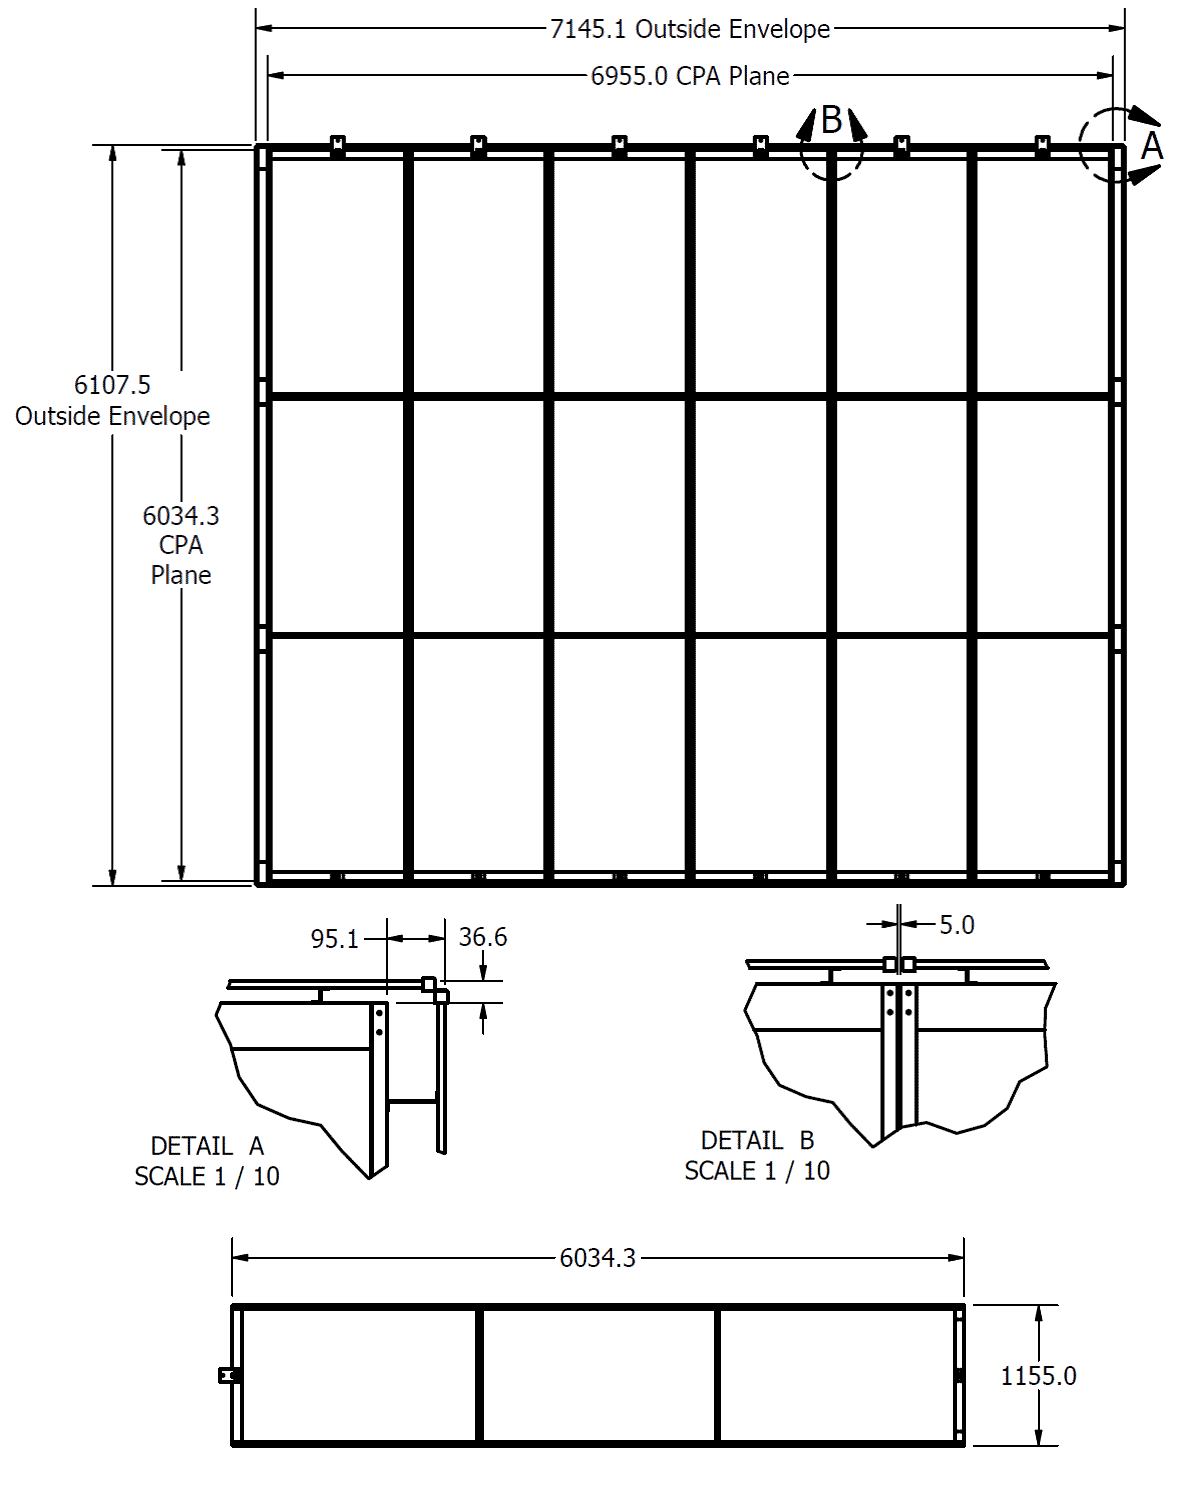
\includegraphics[width=\linewidth]{tpc_cpa_front_views1.png}
\end{cdrfigure}

\begin{cdrfigure}[CPA views2]{cpa-view2}{Views of various part of the CPAs} 
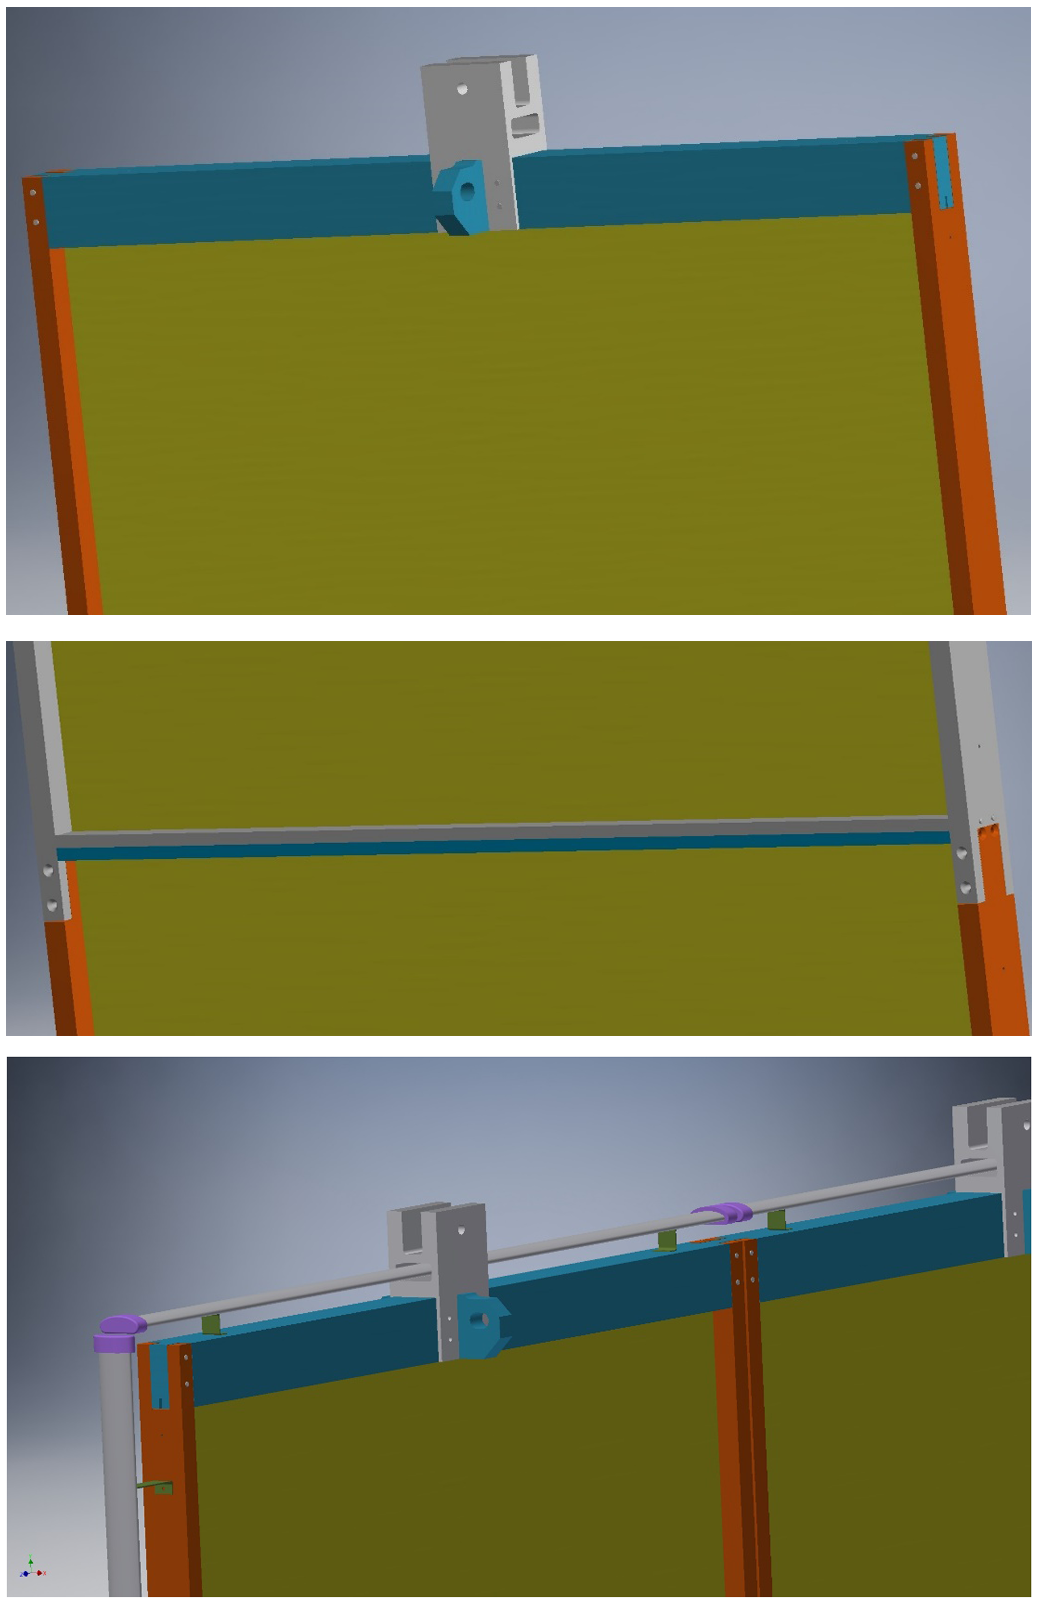
\includegraphics[width=0.8\linewidth]{tpc_cpa_views2.png}
\end{cdrfigure}


Figures~\ref{fig:cpa-geometry} and \ref{fig:cpa-view2} show the basic geometry of the CPA.  The CPA is composed of three modules that are bolted and pinned together with tongue/groove joints to form the full CPA plane.  Each module consists of a framework in which the resistive panel is captured inside a groove.  Each module weights roughly 53~lbs., for a total weight of 160~lbs for a CPA plane.  

The resistive panel is 1/8-inch thick G10 and floats within the framework so that no external forces are applied to it.  When hung vertically the weight of the resistive panel ($\sim$30~lbs per module) rests on the bottom cross bar of the module.  The weight of the modules is transferred through the side bars of the frame  up to the top cross bar, see Figure~\ref{fig:cpa-view2}a.  The very top cross bar of the CPA plane has a block attached to it through which all of the load is transferred to the strap that attaches to the supporting stainless steel I-beam.  

Figure~\ref{fig:cpa-hinge1} shows how the FC will be attached to the assembled CPA plane.  The top and bottom cross bars have elongated slots through which pins are inserted to attach the hinged connection.  The weight of the FC, currently estimated to be 440~lbs., is applied to the center of each top and bottom bar.  

\begin{cdrfigure}[CPA and FCA hinged connection]{cpa-hinge1}{The top field cage modules are hung vertically with the CPAs when moved into the cryostat, then rotated to horizontal to attach to the APA.} 
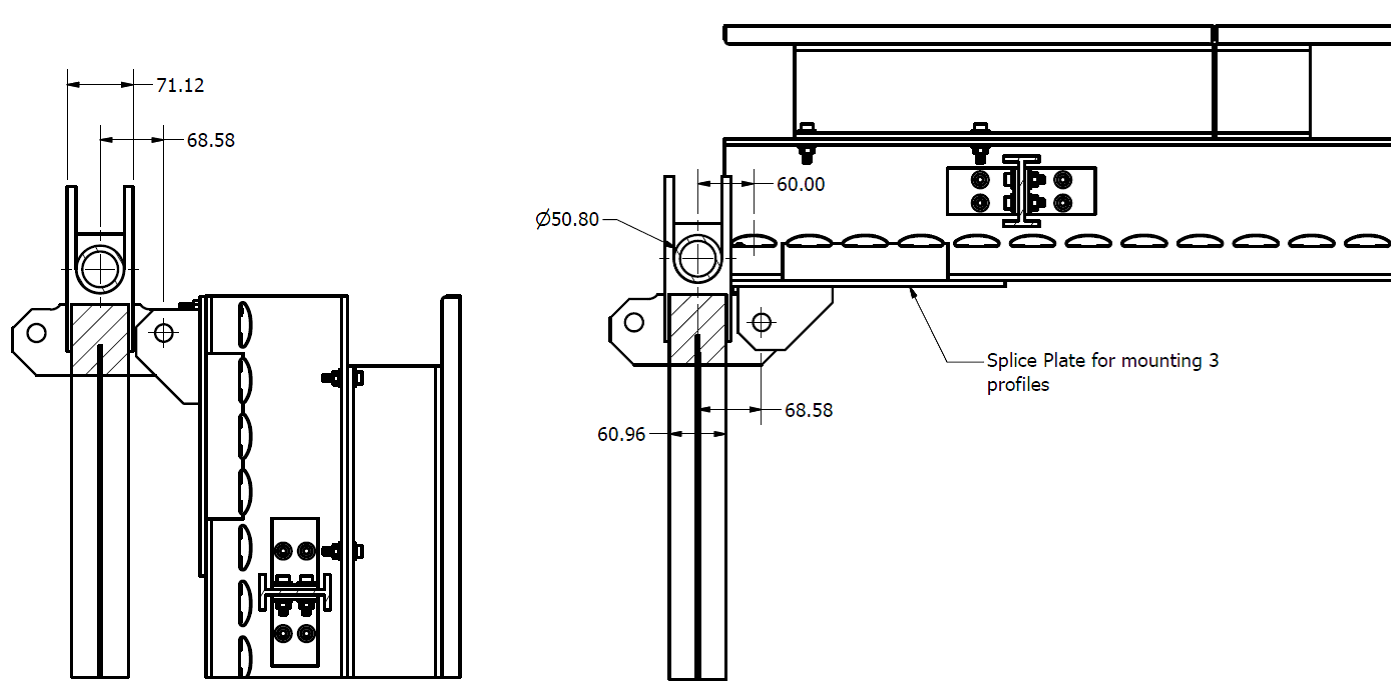
\includegraphics[width=\linewidth]{tpc_cpa_fc_hinge.png}
\end{cdrfigure}


Figure~\ref{fig:cpa-view2}a shows the block at the top of the CPA that is secured to the top cross bar and extends to the top supporting I-beam.  This strap must support the weight of four half FCs (4$\times$220 lbs) and the weight of the CPA itself (160~lbs) for a total weight of 1041~lbs. The section of G10 that connects to the CPA requires and area of only 0.33 in$^2$ to achieve a safety factor of 10 relative to the ultimate strength of the G10.  

The strap must have the ability to allow the CPA to pivot and rotate in three directions.  


The CPA frame has been evaluated using empirical and FEA calculations.  The resistive panels were not included in the analysis. The following is a summary of six key aspects of the analysis. Detailed calculations are shown in 
\fixme{reference to Vic's writeup}.  

%The highest stresses and deflections occur during assembly before the cryostat is filled with liquid.  During installation the CPA must carry the full weight of the FC rather than sharing it with the APA and the buoyancy force which reduces the load from gravity is not present.
The highest stresses and deflections occur during assembly before the cryostat is filled with liquid (when no buoyancy force is present) and the CPA must carry the full weight of the FC.

%In all of the analysis the resistive panels were not included.  In the design of the CPA it is planned that the resistive panel will float within a frame and no load will be applied to it and therefore it does not contribute to the stiffness of the modules.  



{\it A. Lifting the CPA during installation}

%During installation the three frames that make up a CPA module will be placed horizontally on the floor and connected together.  The top of the module will then be secured to the crane and lifted; the bottom of the module will be pivoted on the floor.  By lifting and transversing the hook attached to the top of the module the CPA will be lifted into the vertical position.  
%The worst case loading occurs immediately after the crane begins to lift the top of the module when it is simply supported at the bottom and top.  The stresses and deflections are small as see in Figure~\ref{fig:cpa-h_load}.   The plane will sag a maximum of roughly 2'' and the stresses are below 2,000psi which is far below the ultimate stress.  

During installation the three frames that make up a CPA module will be placed horizontally on the floor and connected together.  To rotate it to vertical, the top of the module will then be secured to the crane and lifted; the bottom of the module will be pivoted on the floor.  The highest loading occurs immediately after the crane begins to lift the top of the module when the CPA is supported only at the bottom and top, but Figure~\ref{fig:cpa-h_load} shows that the stresses and deflections are small.   The plane will sag a maximum of roughly 2~in and the stresses are below 2,000~psi; this is far below the maximum sustainable stress.  

\begin{cdrfigure}[CPA stress in horizontal position]{cpa-h_load}{Stress and deflection of a connected three-CPA stack in horizontal position, supported at both ends} 
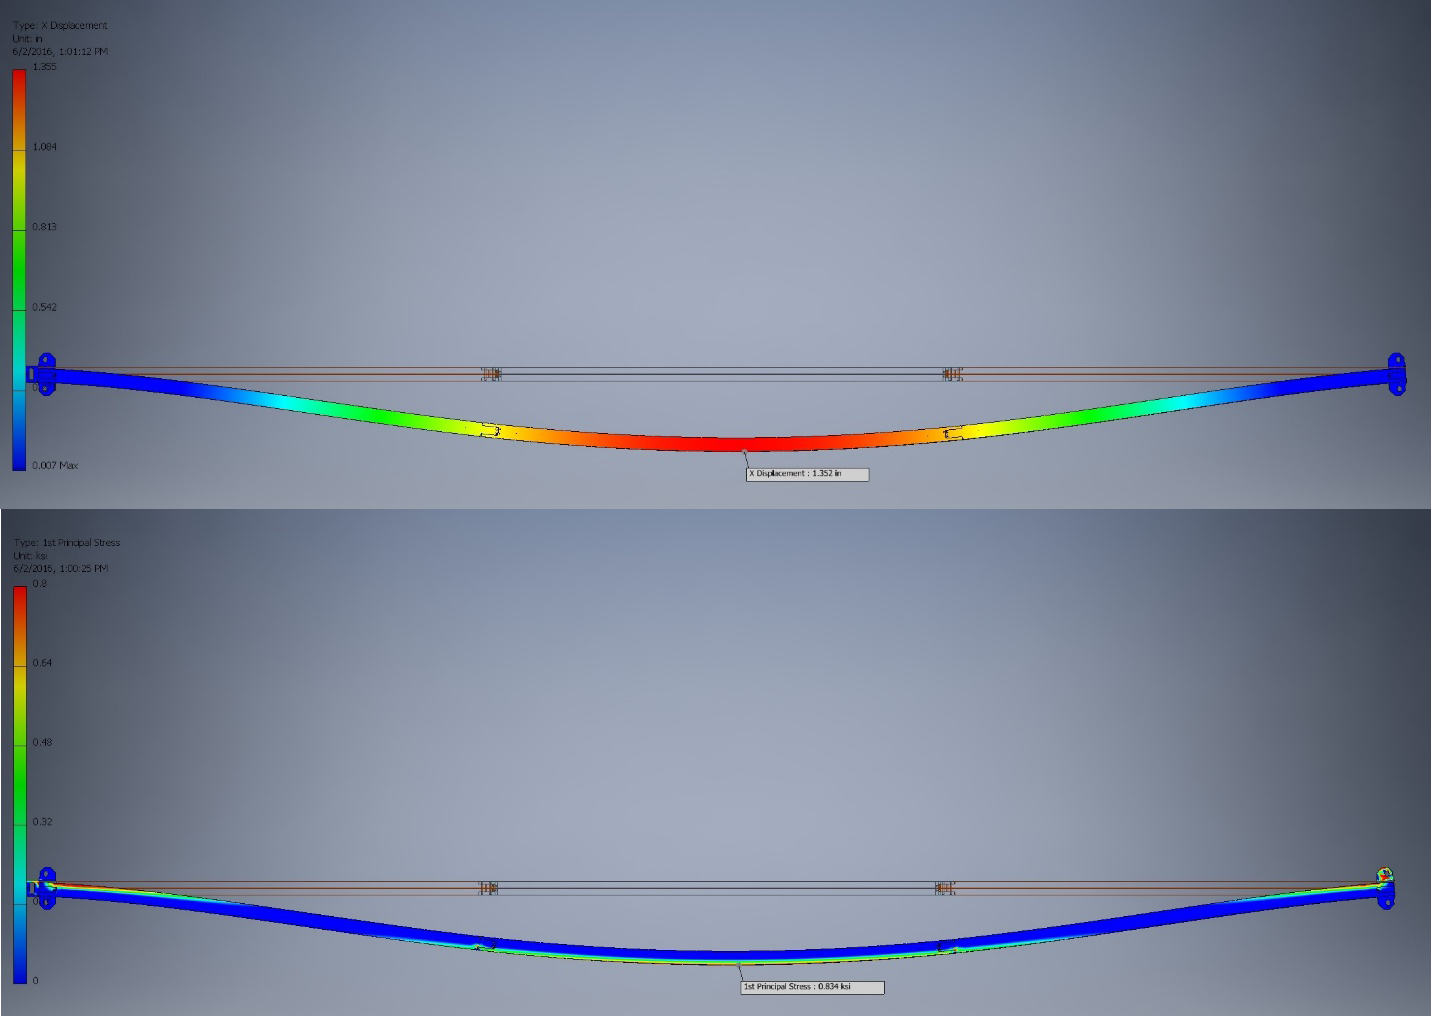
\includegraphics[width=\linewidth]{tpc_cpa_h_load.png}
\end{cdrfigure}


{\it  B. CPA hanging with FC attached in installation position}

%The current estimate for the FC weight is 440 lbs.  This load is carried by 2 CPAs so each hinge on the CPA will supposed 220 lbs in the installation position.  Figure~\ref{fig:cpa-load1} below shows the deflections and maximum stresses.  The larges deflections are at the bottom cross bar of 0.07'' and the stresses are less than 2,000psi which is far below the ultimate stress of G10.

In the installation position the FC weight (440~lbs.) is carried by two CPAs, so each hinge on the CPA will supports 220~lbs.  Figure~\ref{fig:cpa-load1}  shows the deflections and maximum stresses.  The largest deflections (0.07~in) are at the bottom cross bar and the stresses are less than 2,000~psi, which is far below the G10 stress rating.

\begin{cdrfigure}[CPA and 4 FCA load]{cpa-load1}{Stress and deflection of a connected three-CPA stack suspended on the rail with four FC modules} 
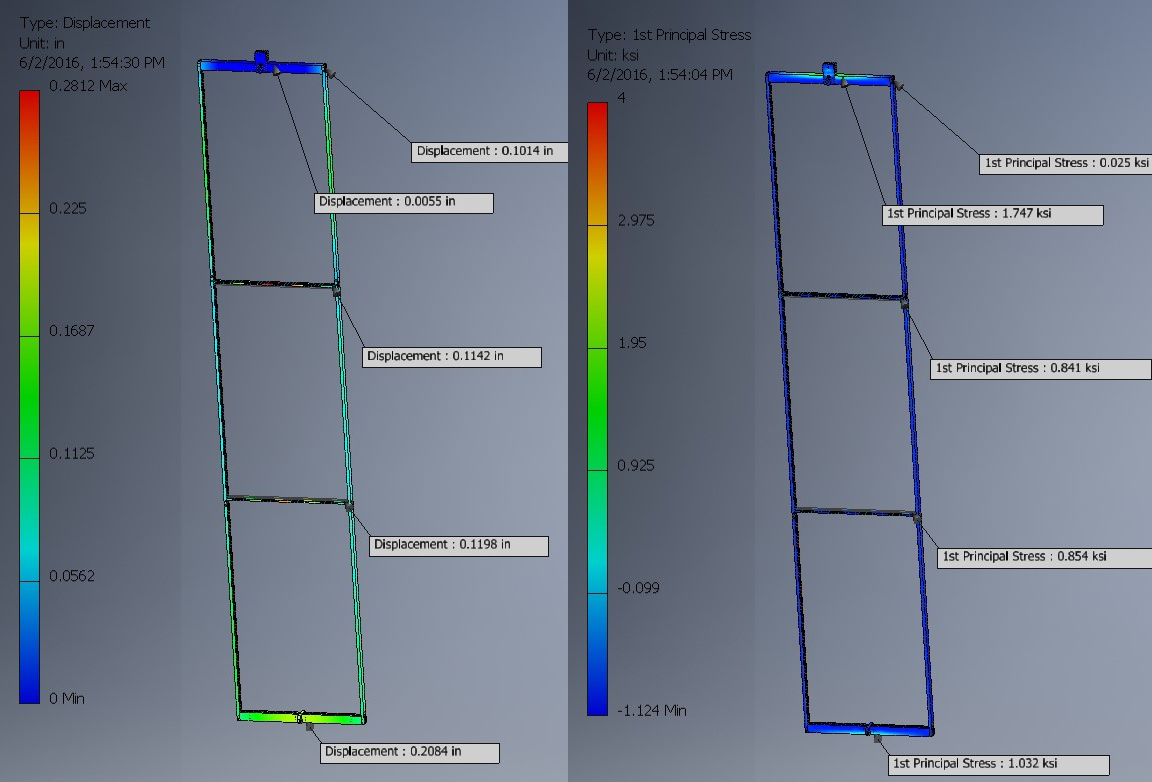
\includegraphics[width=\linewidth]{tpc_cpa_fc_load1.png}
\end{cdrfigure}


{\it  C. CPA hanging with FC attached in deployed position, with weight of worker on FC}

%The current estimate for the FC weight is 440 lbs.  This load is carried by 2 CPAs and by the APAs so each hinge on the CPA will supposed 110 lbs in the installation position.  In addition, in the worst case a 200 lbs worker could be standing directly over an I-beam on the FC directly next to a CPA.  The top two hinges on the CPA will have 110 lbs applied.  One of the bottom hinges will have a 110 lbs load also and the second bottom hinge will have 110 lbs of the FC plus the 200 lbs of the worker applied.  The largest deflection is 0.1'' at the bottom cross bar and the stresses are less than 2200psi which is far below the ultimate stress of G10.

In the deployed position the FC weight  is carried by two CPAs and by the APAs and each hinge on the CPA therefore supports 110~lbs.   The top two hinges on the CPA will need to also support the weight of a worker, estimated to be 200~lbs.; this load is maximized when the worker stands directly over an I-beam on the FC directly next to a CPA, producing a maximum deflection of 0.1~in at the bottom cross bar and stresses less than 2,200~psi, again far below the G10 stress rating.

\begin{cdrfigure}[CPA load plus 200lb]{cpa-load2}{Stresses and deflections of CPA with FC peployed and 200~lb worker load} 
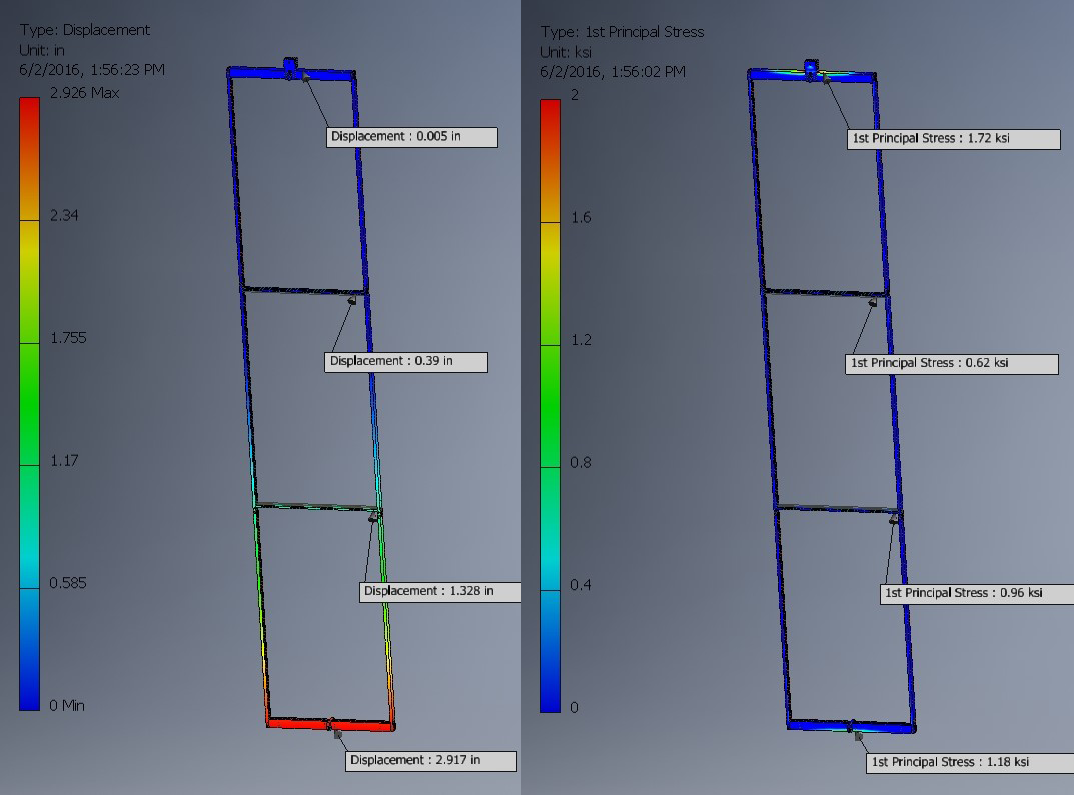
\includegraphics[width=\linewidth]{tpc_cpa_fc_load2.png}
\end{cdrfigure}

{\it D. Connection stresses}

The weight of the CPA and the bottom FC is transferred through the side bars of the CPA frame.  The connection between the side bars and the top cross bar therefore will experience the highest loads.  A single 1/4~in diameter G10 pin at the connection would have a shear stress of 7740~psi; this provides a safety factor of greater than 4.  A second pin at each connection would increase the safety factor to 8.  

{\it E. Deformation and Stress Due to Pressure from Circulating Liquid Argon}

Calculations done at Fermilab indicate that a uniform 2-Pa pressure during cool down will be applied to the resistive panels  %Calculations show 
and that this will result in 0.090-inch deflections of the panel at its center.  The CPA/FC/APA assembly will displace 8.8~mm laterally as a result of the next force from this pressure.  \fixme{next force?}

{\it F. Thermal considerations}

When the CPA modules are cooled, their width will shrink by 0.9~mm.  The supporting stainless steel beam will shrink by 1.6~mm over the width of the CPA.  If the CPA supports are rigidly attached to the supporting stainless steel beam, then an interference of 0.7~mm (the difference) will occur.  To prevent this interference and ensure contact between CPAs after cooldown, an initial gap of 0.7~mm between CPAs is required.  

The steel beam between the CPA and APA will cool and shrink by 5.2~mm.  The joint between the FC and the CPA must be able to accommodate this shrinkage.



%%%%%%%%%%%%
\subsubsection{The mechanical and electrical interconnect features between modules}

%A stack of three modules are interconnected 
Three modules are stacked vertically to form the 6-m height of the ProtoDUNE-SP  cathode.  The frames of these modules are bolted together using tongue-and-groove connections at the ends. The resistive cathode sheets and the field-shaping strips are connected using a few metallic buttons to ensure redundant electrical contact between vertical modules.

There are six columns of the 6-m tall CPA modules in  ProtoDUNE-SP.  Each column is suspended from the CPA rail using a central lifting bar.  Due to the  roof movement between the warm and cold phases of the cryostat, each column is expected to move $\sim$2~mm relative to its neighbors.  Several pin-and-slot connections are implemented at the long edges of the CPA columns to ensure the co-planarity of the modules and yet allow small vertical displacement.  The HV bus interconnects the resistive cathode surfaces across the columns to maintain a uniform voltage across the cathode surface.

%%%%%%%%%%%%%%%%%%%%%%%%
\subsection{QA and QC}

The following activities are planned to assure the CPA meets all design requirements as defined in the fabrication drawings and description in the sections above:
\begin{itemize}
\item Fabricate four prototype CPAs to test the design and fabrication and assembly methods.
\item Installation test at Ash River:
\begin{itemize}
\item Test the lifting and handling of the four prototype CPA’s.
\item  Load the 4 prototype CPA’s with FC modules and test and evaluate their installation.
\end{itemize}
\item Develop a QC plan for inspecting every fabricated part of the CPA frame to make sure they meet the dimensions and tolerances on the fabrication drawings.
\item Develop a QC plan for inspecting and measuring each CPA module and completed CPA plane to ensure they meet the dimensions and tolerances on the drawings.
\item Perform tests of each joint in the CPA frame (see Section 3) to ensure that their design and strength meets the load requirements.
\item Create an integrated model of the entire TPC to evaluate interfaces and installation methods.  
\item Develop a QC for receiving the resistive panels.  Measure the dimensions to confirm they meet the drawings and setup a plan and acceptance criteria to insure that panel resistance is acceptable.
\item Develop a QC  HV test at CERN for evaluating side to side and top to bottom resistance for each completed CPA but after final assembly and after hanging during installation.  
\item Performed 35 ton HV test at FNAL.
\end{itemize}


